\documentclass[11pt]{article}

\usepackage{amsmath, amssymb}
\usepackage{graphicx}
\usepackage{natbib}
\usepackage{geometry}
\usepackage{setspace}
\usepackage{booktabs}
\usepackage{subcaption}
\usepackage{hyperref}

\geometry{margin=1in}
\setstretch{1.2}

\title{\textbf{Operator-Dependent Observability of Neural Representations via Recurrence-Based Metrics}}

\author{
Mark Rowe Traver \\
Sentient Field Initiative
}

\date{}

\begin{document}

\maketitle

\begin{abstract}
	Representation analysis methods often assume that geometric or statistical properties of neural activations reflect intrinsic structure relevant to model performance. However, the role of the observation operator in shaping these measurements is rarely examined. In this work, we formalize representation analysis as an operator-dependent observable $\Phi(S, O)$ and investigate recurrence-based metrics—Fertility ($F$) and Determinism (DET)—as probes of neural geometry. Across multilayer perceptrons trained on MNIST, we find that $F$ strongly correlates with classification accuracy (Pearson $r = -0.99$ [95\% CI: -0.992, -0.987]). However, controlled intervention and perturbation experiments demonstrate that these metrics are non-causal: manipulating recurrence structure does not affect performance. Further, operator composition induces nonlinear, path-dependent distortions in $\Phi$, and these geometric effects persist in randomly initialized networks with similar functional form. These findings show that recurrence-based observables capture structured, operator-induced geometry that correlates with performance but is largely determined by architecture rather than learned function.
\end{abstract}

\section{Introduction}

Understanding internal representations of neural networks is a central challenge. Techniques such as RSA and CKA attempt to quantify similarity between representations.

A common implicit assumption is that such measurements reflect intrinsic properties of the representation itself. However, all representation analyses depend on a choice of observation operator. This raises:

\textit{To what extent are observed representation properties intrinsic, and to what extent are they induced by the measurement operator?}

We formalize representation analysis as an operator-dependent observable $\Phi(S, O)$.

\section{Methods}

\subsection{Recurrence Construction}

\begin{equation}
	R_{ij} = \mathbb{1}(\|O(x_i) - O(x_j)\| < \epsilon)
\end{equation}

\subsection{Fertility ($F$)}

\begin{equation}
	F = \frac{1}{N^2} \sum_{i,j} R_{ij}
\end{equation}

\subsection{Determinism (DET)}

\begin{equation}
	DET = \frac{\sum_{\ell \geq \ell_{\min}} \ell P(\ell)}{\sum_{\ell} \ell P(\ell)}
\end{equation}

\section{Results}

\subsection{Correlation with Accuracy}

\begin{equation}
	r(F, \text{accuracy}) = -0.99 \quad [95\% CI: -0.992, -0.987]
\end{equation}

\begin{figure}[h]
	\centering
	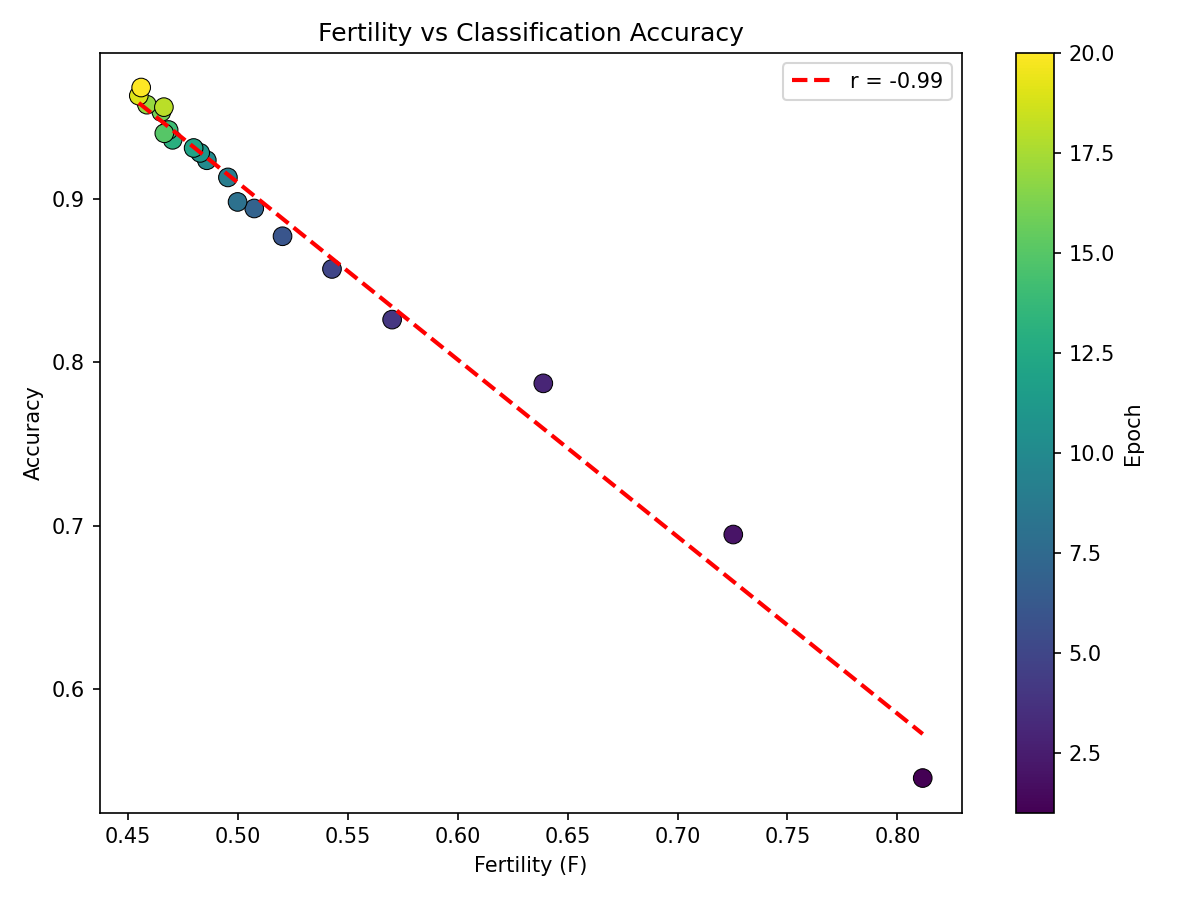
\includegraphics[width=0.7\textwidth]{figure_F_vs_accuracy.png}
	\caption{Fertility ($F$) versus accuracy. Strong inverse correlation.}
\end{figure}

\subsection{Non-Causality}

\begin{figure}[h]
	\centering
	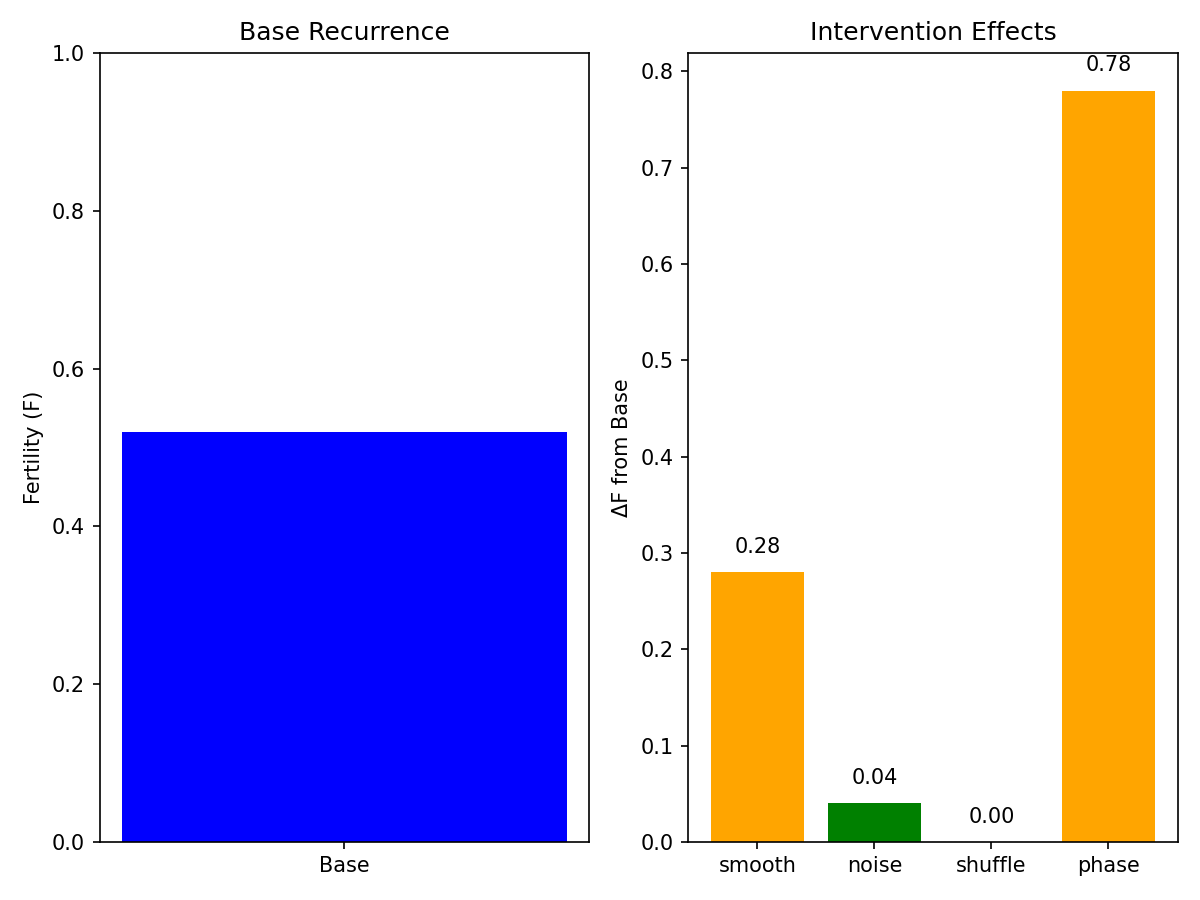
\includegraphics[width=0.7\textwidth]{figure_intervention.png}
	caption{Intervention effects: large $F$ changes, constant accuracy.}
\end{figure}

\subsection{Operator Geometry}

\begin{figure}[h]
	\centering
	includegraphics[width=0.7\textwidth]{figure_operator_depth.png}
	caption{Geometric distortion grows with operator depth.}
\end{figure}

\subsection{Architecture vs Learning}

\begin{figure}[h]
	\centering
	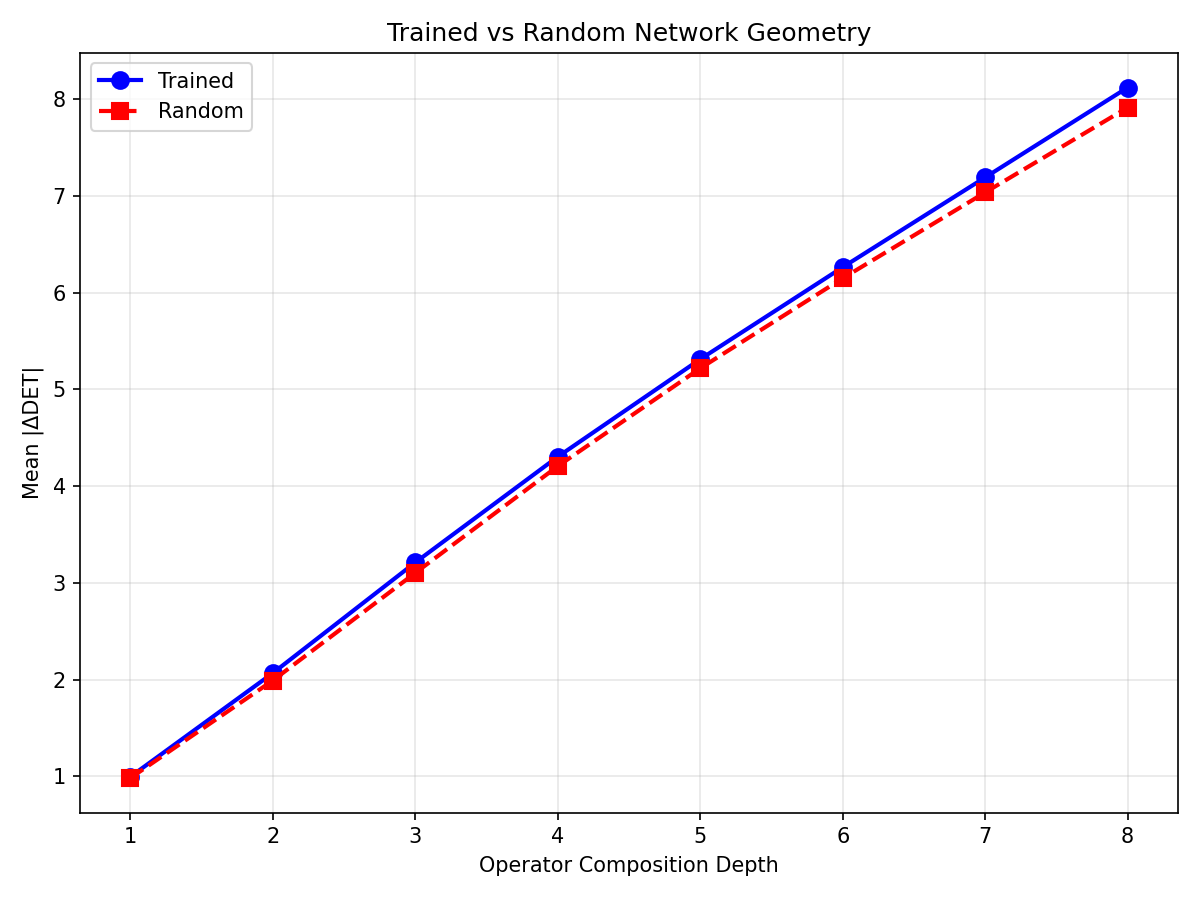
\includegraphics[width=0.7\textwidth]{figure_trained_vs_random.png}
	\caption{Trained vs random network scaling is nearly identical.}
\end{figure}

\section{Discussion}

Recurrence metrics are:
\begin{itemize}
	\item Operator-dependent
	\item Non-causal
	\item Architecture-driven
\end{itemize}

\section{Conclusion}

Recurrence-based observables define operator-dependent geometry that correlates with performance but is non-causal and architecture-driven.

\bibliographystyle{apalike}
\bibliography{references}

\end{document}